\documentclass[a4paper, 11pt, oneside]{article} % A4 paper size, default 11pt font size and oneside for equal margins

\usepackage[utf8]{inputenc} % Required for inputting international characters
\usepackage[T1]{fontenc} % Output font encoding for international characters
\usepackage[french]{babel}
\usepackage{csquotes}

\usepackage[twoside, margin=2.5cm, bindingoffset=0.0cm]{geometry}

\usepackage{hyperref} %For hyperlinks 
\hypersetup{pdfborder=0 0 0}

\usepackage{graphicx}  % Pour images
\graphicspath{{Figures/}}

\usepackage[%backend=biber,
style = ieee,
sorting=none
]{biblatex} %,bibstyle=ieeehttps://www.overleaf.com/project/624dc5f129c1767e8bb8de67
\addbibresource{biblio.bib}
\renewbibmacro*{date}{%
  \iffieldundef{year}
    {\bibstring{nodate}}
    {\printdate}
}

\newcommand{\comment}[1]{}%pour faire des comentaires a plusueures lignes 
\newcommand{\dd}[1]{\mathrm{d}#1}
% TODO trouver une meilleure alternative que ca car ca enleve litalique et apres faire renewcommand \vb*{\}\(
    
\usepackage{physics} %pour \vb*{b}old vectors
%\newcommand{\vb*}[1]{\boldsymbol{#1}}
%\newcommand{\vb*}[][]{}
\begin{document} 
\tableofcontents
\listoffigures
\listoftables
\section*{Introduction}
    % Dire cest quoi leffet cheerios etc \ldots
    %What are cheerios? Is the cheerios effect really an effect or something we created in our reality to rationalise the sogyness of our cereals. Will we be able to eat cereals without making them soggy since we will be so foccused at the cheerios effect. Is the cheerios effect a conspiracy fro cheerios to make us eat soggy cereals or mayb ethey are thirsty and want more time in liquid or maybe they miss their friends inside the bag so the y curve the water to reach them but there was something that they didnt know; the fact that researchers would modelise it and one day two students would choose this effect do simulate it. Maybe that was the objective overall trying to put sense in our worthless lifes. Why would the cheerios be intersted in our lifes? Are we interested in our lifes? Who knows \ldots  
    %Maybe one day we will see what this project meant to but for now we are sailing sailing on the unexpected and in a world filled with possibilities only exploring some possibilities leaving infinite ones untouched. Maybe one day all that will make sense but for now the only thong that makes sense is this paper or maybe not even this so would that mean that our life doesnt have sense/meaning? That is left to the reader maybe it does maybe it doesn't. Maybe it depends how you look at it. It is all filled with maybes however you might look at it as someone scottis and i quote "No you you seee i'm talking facts here i dont do if buts and maybes i do absolutes..." and in that case i have only one thing to say in this paper that should be the case. And with all that said i am leaving you with this paper and a little bit of existentialism, nihilism and our besst wishes about the future.

    Dans le cadre de l'UE Projet en Calcul Scientifique Numérique, nous devions travailler sur un projet, afin de nous apprendre plus en détail, la programmation et le calcul numérique avec un langage compilé, le C. Notre sujet était sur l'"Effet Cheerios", ou l’intéraction d'objets à la surface d'un liquide par l'effet de la gravité et la déformation interfaciale. Cet effet se caractérise par la tension d'une surface liquide sous le poids d'un objet, par exemple une punaise sur l'eau. Lorsque nous ajoutons plusieurs objets sur la même surface, à distance plus ou moins grande, les objets vont potentiellement s'attirer puis créer des tas mobiles. Ce phénomène est notamment visible avec des céréales dans du lait, d'où le nom de Cheerios, célèbre marque de céréales américaine. Pour réaliser à bien ce projet nous avons du faire de nombreuses recherches sur la mécanique des fluides, les collisions inélastiques et nous avons également du faire un travail conséquent sur l'optimisation de notre algorithme.

\section{Le problème et notre modélisation}
    % TODO pas sur mais ca peux etre sympa si on se focus plus a cheerios que ceci est pour un cours peut etre ? je sais pas ? qui sais ? pas moi en tot cas. 
On a tous mange des ceriales ou vu des objets flottant atirer vers ou pouse par eux; mais cest quoi la raison de cette force dans ce projet cree au sein de l'UE projet en calcul scientific on a fait la simulation des objets flottants.

TODO faire un tableau de symboles que on utilise comme \(\gamma\) surface tension etc

\begin{table}
    \centering
    \begin{tabular}{ccc}
        \hline
        abraviation & nom & dimension\\
        \hline
        $R$      & Rayon de courbure & TODO\\
        $\gamma$ & surface tension   & TODO\\ 
        $\rho_s$ & densite solide    & TODO\\
        $\rho_l$ & densite liquide   & TODO\\
        $\rho_a$ & densite air       & TODO\\
        $B$      & nombre de Bond    & TODO\\
        \hline
    \end{tabular}
    \caption{Table des variables}
\end{table}

\subsection{Effet Cheerios}
    Cette partie est plutot fait pour lintegrite du rapport le lecteur est fortement encourage a lire \cite{vella_cheerios_2005} pour avour une plus complete comprehension du sujet \textit{cheerios effect}
    Les formules pour les calculs viennent principalement de \cite{vella_cheerios_2005}
    TODO expliquer de ou viens les forces des angles qui tord la surface ?

    Expliquer leffet de cheerios.
    
    % TODO peut etre notre propre figure ?
    \begin{figure}
        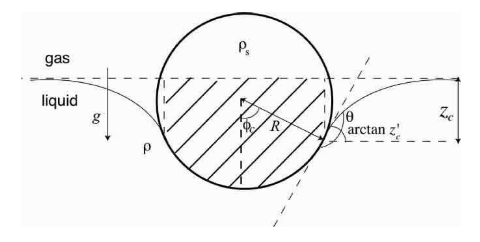
\includegraphics[width = 0.9\textwidth]{boulleflotantedecheerios.png}
        \caption{Geometry of a sphere lying at a liquid-gas interface. The shaded area represents the weight of liquid equivalent to the buoyancy force due to hydrostatic pressure acting on the sphere.\cite{vella_cheerios_2005}}
    \end{figure}
    Une des raisons la quel les objets flotte cest due a la pusee de archimede et ces't un des cas majeurs dans notre probleme aussi. Comme on peux voir dans la figure TODO metre la citation de la figure en haut.
    
    Pour que notre sphere reste sur linterface il a besoin que son poids \(\frac{4}{3}\pi\rho_{s}gR^3\) devrait etre en equilibre par la composante de pousee de archimede a lendroit de contact du liquide avec la sphere et la force de tension sur la surface ??? must be balanced by the component of surface tension acting along the (circular) contact line and the buoyancy force because of the displaced bulk fluid.

    TODO expiquer dou ca viens moi ja pas comprie
    \begin{equation}
        2\pi R \phi_c \gamma \sin(\arctan z_c^{'}) = 2\pi\gamma R \sin\phi_c z_c^{'}(1+z_c^{'2})^{-1/2}
        \label{eq:wut}
    \end{equation}

    Buoyancy force
    \begin{equation}
        \pi\rho_l g R^3 (\frac{z_c}{R}\sin^2 \phi_c + \frac{2}{3}-\cos\phi_c+\frac{1}{3}\cos^3 \phi_c)
        \label{eq:buoyancyForce}
    \end{equation}

    Balance of vertical forces
    Alors on a
    \begin{equation}
        \Rightarrow \frac{4}{3}\pi\rho_{s}gR^3 =2\pi\gamma R \sin\phi_c \frac{z_c^{'}}{\sqrt{(1+z_c^{'2})}} + \pi\rho_l g R^3 (\frac{z_c}{R}\sin^2 \phi_c + \frac{2}{3}-\cos\phi_c+\frac{1}{3}\cos^3 \phi_c)
    \end{equation}

    TODO cest quoi $z_c^{'}$???

    Si on substitue \(\phi_c = \pi - \theta + \arctan z_c^{'}\) et garde seulement les termes linear en \(z_c^{'}\) on retrouve l'expression pour \(z_c^{'}\sin \phi_c\) qui est precis a \textit{linear order in the Bond number} \(B \equiv R^2/L_c^2\) 

    Alors on a:
    \begin{equation}
        z_c^{'}\sin \phi_c = B(\frac{2D-1}{3}-\frac{1}{2}\cos \theta + \frac{1}{6} \cos^3 \theta) \equiv B\Sigma
        \label{eq:bondsigma}
    \end{equation}
    Avec \(D \equiv \rho_s / \rho\) On peux voir ceci est bien le cas car on observe bien que \(z_c^{'} = 0\) quand \(\theta = \pi/2\) et \(D = 1/2\) cest ce que on satendais car dans ce cas la pousee de archimede seul lui meme est assez pour equilibrer le poids de la sphere sans deformations du liquide.

    L'equation\ref{eq:bondsigma}contient deux parametres sans dimensions; \textit{Bond number}$B$ et $\Sigma$ tres importants pour notre modélisation.

    \begin{equation}
        B = \frac{(\rho_l-\rho_{a})gR^2}{\gamma}
    \end{equation}
    Le nomre de Bond nous donne la mesure relative de limportance des effets de gravite et tension de surface; si $B$ est tres grande ca correspond a des particules grandes ou une tension de surface petit. 

    WUT ????

    The expression for the slope of the interface in the vicinity of the spherical particle given in (9) is valid for B << 1 (corresponding to a radius of  1mm or smaller for a sphere at an air-water interface) in which case surface tension is very important. The other dimensionless parameter, , can be thought of as a (non-dimensional) resultant weight of the particle once the Archimedes upthrust has been subtracted out. This physical interpretation arises naturally from the vertical force balance condition (8) and (9) since the resultant weight of the object (in the linearised approximation) is simply 

    To calculate the interaction energy using the Nicolson
    approximation, we must also calculate the interfacial displacement caused by an isolated floating sphere, which is determined by the hydrostatic balance gamma nabla²h = rho gh - the co-ordinate invariant statement of equation (1). With the assumption of cylindrical symmetry, this becomes:
    \(\gamma \nabla^2h = \rho_l g h\)
    \begin{equation}
        \gamma \frac{\dd^2h}{\dd x^2} = \rho_l g h
    \end{equation}
    Si on assume une symetrie spherique
    \begin{equation}
        \Rightarrow \frac{1}{r} \frac{\dd}{\dd r} \left( r\frac{\dd h}{\dd r}\right) = \frac{h}{L_c^2}
    \end{equation}
    TODO developer bessel
    \cite{introtoBessel}

    % TODO dans le code ajouter un buoyancy force qui calcule la ousee de archimede et dis si notre objet flotte ou pas si il flotte pas on peux metre un option tel quel il prend la valeur automatique ??? Ou on le neglige ????
    % TODO On mets les formules et peut etre demontrer ou ils viennent et surtout les cas ou on peux utiliser ces formules les cas ou ca marche pas etc\ldots
    % TODO SCHEMA deux cheeios et sur le schema on monre l Rayon de courbure etc...
    % TODO graphique des foncions de bessel
    % TODO citer cheerios 
    \begin{equation}
        \label{ForceEntreCheerios}
        F(l) = -2\pi \gamma R B^{5/2} K_1 \left( \frac{l}{L_c}\right)
    \end{equation}

        
        \subsection{Collsisions}
        Expliquer comment on a deduit que les collisions etait des collisions inelastic parfait et metre les equations utilise
        Pour les collisions, nous sommes partis sur un modèle assez simple qui itère chaque objet et regarde si la distance entre eux est plus petite que leur rayons additionnés on dis que il ya une collision et on applique les collisions et la conservation de momentum.
        \begin{itemize}
            \item Dabord on prend le vecteur norme collisions qui est le sens de 1 a 2 $\vb*{c} \longrightarrow ||\vb*{c}|| = 1$ 
            \item Apres on trouve la vitesse relative pour voir comment les cheerios vont saffecter
            \item Et on calcule la vitesse avec le produit scalaire de vitesse relative et la norme de collision ceci ca va nous etre utile quand on calcule m'impulse des objets $\vb*{v_{collision}}=\vb*{v_{relative}}\vb*{c} $
            \item et on aplique un coefficient entre 0.2 et 0.7 car notre experience nest pas des collisions elastique parfaite. Par contre il faux faire aatention a cette constante car si on le mets trop petit ca fait tel que les cheerios na pas le rebond nescesaire et comence a entrer dans eux et si on le mets trop eleve ca fait tel que ca rebondit beaucoup mais tout ces effects negative diminue plus on prend notre pas de temps petit
            \item si la vitesse de collision est plus grand que 0 ca veux dire ils vont vers eux meme donc une collision ???? ca veux dire que autremenet meme si ils sont entre eux il ya pas de collision ???? revoir applique collision et le if
            \item on calcule limpulse $i = 2\frac{v}{m_1 m_2}$
            \item et on soustrait la vitesse du cheerio 1 par $\vb*{v_1} -= i*m_2*\vb*{c}$
            \item et on ajoute pour lautre $\vb*{v_2} -= i*m_1*\vb*{c}$
        \end{itemize} 
        \section{Méthodes numériques et algorithme}
        \subsection{Integration de Verlet}
            Pour déterminer nos coordonnées, vitesses et accélérations en fonction du temps nous avons opté pour l'intégration de Verlet. L'intégration de Verlet est un algorithme simple à mettre en place et qui permet de conserver l'énergie dans le système. L'algorithme utilise le développement limité de Taylor de notre vecteur position à l'ordre 3.

            %On prouve lintegration de verlet et montre que on peux lutiliser pour notre probleme
            %Si on applique le developement limite de x on peux deduir les positions suivant
            Démonstration du développement limité de Taylor Young de $f(x)$ au point $x_0$\cite{agarwal_introduction_2011} :% TODO citer le livre de introduction a lanalyse complexe et numerique dans la mir 
            \begin{equation}
                DL_n f(x) = \sum_{i=0}^{n}\frac{f^{(i)}(x_0)}{i!}(x-x_0)^i+ o((x-x_0)^n)
            \end{equation}
            Si on applique le développement limité d'ordre 3 à la position($\vb*{x}(t+\dd t)$) au point $t+\dd t$ on a l'équation suivante avec $t_0$ comme le pas de temps précédent :
            % On a ca avec le developement limilte a $t$ et $t_0$ cest le pas temps precedent
            \[DL_3 \vb*{x}(t) = \vb*{x}(t_0)+\vb*{x}^{'}(t_0)(t-t_0)+\frac{\vb*{x}^{''}(t_0)}{2!}(t-t_0)^2 +o((t-t_0)^3)\]
            Si $t_0$ est le pas de temps précédent, $\vb*{x}^{'}(t)$ vitesse et $\vb*{x}^{''}(t)$ l'accélération, nous avons :
                \[DL_3 \vb*{x}(t+\dd t) = \vb*{x}(t)+\vb*{x}^{'}(t)(t+\dd t-t)+\frac{\vb*{x}^{''}(t)}{2!}(t+\dd t-t)^2+o(t+\dd t-t)\]
                \[\Rightarrow DL_3 \vb*{x}(t+\dd t)= \vb*{x}(t)+\vb*{v}(t)(\dd t)+\frac{\vb*{a}(t)}{2!}(\dd t)^2+o(\dd t^3)\]
            L'erreur sur le temps $t_n$ est de l'ordre de $o(\exp^(Lt_n)\dd t^2)$ % TODO pas sur de ici
    
            Notre accélération ne dépendant pas du changement de vitesse mais de l'équation (\ref{ForceEntreCheerios}), nous pouvons calculer l'accélération à partir du principe fondamental de la dynamique avec une masse constante. Il est important de faire cela après le calcul de position mais avant la vitesse car la position prend l'accélération précédente et la vitesse prend celui de avant et pendant le temps.
            \begin{equation}
                \label{PFD}
                \sum  \vb*{F} = m\vb*{a} \Longrightarrow \vb*{a} = \frac{\sum \vb*{F}}{m}
            \end{equation}
    
            Maintenant nous avons la nouvelle position et l'accélération, nous pouvons calculer la nouvelle vitesse.
            % TODO dire dou cette formule viens 
            \begin{equation}
                \label{verletVitesse}
                \vb*{v}(t+\dd t) = \vb*{v}(t)+\frac{\vb*{a}(t)+\vb*{a}(t+\dd t)}{2}\dd t 
            \end{equation}
            % est que on mets ca sur lanexe ?
            % (voir lanexe pour le developement du calcul) 
            %        \[DL_3 x(t+\dd t)= x(t)+x^{'}(t)(\dd t)+\frac{x^{''}(t)}{2!}(\dd t)^2\]
            %= & x(t)+x^{'}(t)(t+\dd t-t)+\frac{x^{''}(t)}{2!}(t+\dd t-t)^2\\
            %Essai avec $x(t)$\[DL x(t) = x(t_0)+x^{'}(t_0)(t-t_0)+\frac{x^{''}(t_0)(t-t_0)^2}{2!}\]
    \subsection{collision des bords}
        Et aussi on fait des collisions de bord aussi.
    \subsection{force des bords}
        pour la force appliquée par les bords sur les objets nous avons décidé de ne pas calculer les forces de chaque point du bord, au lieu de cela nous avons utilisé la symétrie d'un cercle (nos bords étant un cercle). Seulement deux forces de bords vont s'appliquer sur un objet, les autres s'annulant par symétrie, comme le montre la figure \ref{Force_Bord_schéma}
        \begin{figure}
            \centering
            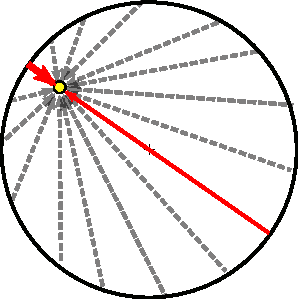
\includegraphics{Figure_Force_Bord.pdf}
            \caption{Schéma des forces des bords.}
            \label{Force_Bord_schéma}
        \end{figure}
        % \begin{equation}
            
        % \end{equation}
        % TODO 


\section{Comment on a concue notre probleme}
    \begin{itemize}
        \item On a pris l'interaction des forces totale sur chaque particule par la fonction dans l'article `Cheerios effect'
        \item et de ca on deduis la force que reagis a chaque cheerios pour un pas de temps 
        \item Check si il ya des collisions ou pas et si il ya on change les proprietes des cheerios par rapport aux collisions
        \item De la force en utilisant l'integration de verlet et le principe fondamentale de la dynamique somme forces = derive (masse*vitesse) on peux changer les positions des cheerios
    \end{itemize}

\section{Les choses a ameliorer}
    \begin{itemize}
        \item Code en $O(NT\cdot n^2)$ et peux etre ameliorer enn$O(NT\cdot n\log n)$ en faisant le calcul de collisions plus inteligament a la place de une recherche exasthive et en calculant une seule fois le \textit{millieu} des forces de chaque particule pour avoir un centre de atraction et comme ca on calcule le centre de attraction regarde si on a des collisions ou pas et a la fin ajoute les forces du bords a chaque particule
        \item pour linstant on utilise les equations \textit{aproximatives} on peux les essayer de les resoudres sans approximations en utilisant laproximation de Nicholson(fine difference method)
        \item le code marche seulement pour les objets ronds faux ajouter une facon plus complexe pour plus de objets
    \end{itemize}
\section*{Conclusion}

% TODO pq la bibliographie ne marche pas ?
\newpage
\thispagestyle{empty}
\nocite{*}
\addcontentsline{toc}{section}{Bibliographie}
\printbibliography[title = Bibliographie]

\end{document}
